\documentclass[man,floatsintext]{apa6}
\usepackage{lmodern}
\usepackage{amssymb,amsmath}
\usepackage{ifxetex,ifluatex}
\usepackage{fixltx2e} % provides \textsubscript
\ifnum 0\ifxetex 1\fi\ifluatex 1\fi=0 % if pdftex
  \usepackage[T1]{fontenc}
  \usepackage[utf8]{inputenc}
\else % if luatex or xelatex
  \ifxetex
    \usepackage{mathspec}
  \else
    \usepackage{fontspec}
  \fi
  \defaultfontfeatures{Ligatures=TeX,Scale=MatchLowercase}
\fi
% use upquote if available, for straight quotes in verbatim environments
\IfFileExists{upquote.sty}{\usepackage{upquote}}{}
% use microtype if available
\IfFileExists{microtype.sty}{%
\usepackage{microtype}
\UseMicrotypeSet[protrusion]{basicmath} % disable protrusion for tt fonts
}{}
\usepackage{hyperref}
\hypersetup{unicode=true,
            pdftitle={Tutorial of network analyses of ESM data: the lagnetw package},
            pdfauthor={Peter Verboon~\& Annelie Beijer},
            pdfkeywords={network ESM lags Multilevel},
            pdfborder={0 0 0},
            breaklinks=true}
\urlstyle{same}  % don't use monospace font for urls
\usepackage{color}
\usepackage{fancyvrb}
\newcommand{\VerbBar}{|}
\newcommand{\VERB}{\Verb[commandchars=\\\{\}]}
\DefineVerbatimEnvironment{Highlighting}{Verbatim}{commandchars=\\\{\}}
% Add ',fontsize=\small' for more characters per line
\usepackage{framed}
\definecolor{shadecolor}{RGB}{248,248,248}
\newenvironment{Shaded}{\begin{snugshade}}{\end{snugshade}}
\newcommand{\KeywordTok}[1]{\textcolor[rgb]{0.13,0.29,0.53}{\textbf{#1}}}
\newcommand{\DataTypeTok}[1]{\textcolor[rgb]{0.13,0.29,0.53}{#1}}
\newcommand{\DecValTok}[1]{\textcolor[rgb]{0.00,0.00,0.81}{#1}}
\newcommand{\BaseNTok}[1]{\textcolor[rgb]{0.00,0.00,0.81}{#1}}
\newcommand{\FloatTok}[1]{\textcolor[rgb]{0.00,0.00,0.81}{#1}}
\newcommand{\ConstantTok}[1]{\textcolor[rgb]{0.00,0.00,0.00}{#1}}
\newcommand{\CharTok}[1]{\textcolor[rgb]{0.31,0.60,0.02}{#1}}
\newcommand{\SpecialCharTok}[1]{\textcolor[rgb]{0.00,0.00,0.00}{#1}}
\newcommand{\StringTok}[1]{\textcolor[rgb]{0.31,0.60,0.02}{#1}}
\newcommand{\VerbatimStringTok}[1]{\textcolor[rgb]{0.31,0.60,0.02}{#1}}
\newcommand{\SpecialStringTok}[1]{\textcolor[rgb]{0.31,0.60,0.02}{#1}}
\newcommand{\ImportTok}[1]{#1}
\newcommand{\CommentTok}[1]{\textcolor[rgb]{0.56,0.35,0.01}{\textit{#1}}}
\newcommand{\DocumentationTok}[1]{\textcolor[rgb]{0.56,0.35,0.01}{\textbf{\textit{#1}}}}
\newcommand{\AnnotationTok}[1]{\textcolor[rgb]{0.56,0.35,0.01}{\textbf{\textit{#1}}}}
\newcommand{\CommentVarTok}[1]{\textcolor[rgb]{0.56,0.35,0.01}{\textbf{\textit{#1}}}}
\newcommand{\OtherTok}[1]{\textcolor[rgb]{0.56,0.35,0.01}{#1}}
\newcommand{\FunctionTok}[1]{\textcolor[rgb]{0.00,0.00,0.00}{#1}}
\newcommand{\VariableTok}[1]{\textcolor[rgb]{0.00,0.00,0.00}{#1}}
\newcommand{\ControlFlowTok}[1]{\textcolor[rgb]{0.13,0.29,0.53}{\textbf{#1}}}
\newcommand{\OperatorTok}[1]{\textcolor[rgb]{0.81,0.36,0.00}{\textbf{#1}}}
\newcommand{\BuiltInTok}[1]{#1}
\newcommand{\ExtensionTok}[1]{#1}
\newcommand{\PreprocessorTok}[1]{\textcolor[rgb]{0.56,0.35,0.01}{\textit{#1}}}
\newcommand{\AttributeTok}[1]{\textcolor[rgb]{0.77,0.63,0.00}{#1}}
\newcommand{\RegionMarkerTok}[1]{#1}
\newcommand{\InformationTok}[1]{\textcolor[rgb]{0.56,0.35,0.01}{\textbf{\textit{#1}}}}
\newcommand{\WarningTok}[1]{\textcolor[rgb]{0.56,0.35,0.01}{\textbf{\textit{#1}}}}
\newcommand{\AlertTok}[1]{\textcolor[rgb]{0.94,0.16,0.16}{#1}}
\newcommand{\ErrorTok}[1]{\textcolor[rgb]{0.64,0.00,0.00}{\textbf{#1}}}
\newcommand{\NormalTok}[1]{#1}
\usepackage{graphicx,grffile}
\makeatletter
\def\maxwidth{\ifdim\Gin@nat@width>\linewidth\linewidth\else\Gin@nat@width\fi}
\def\maxheight{\ifdim\Gin@nat@height>\textheight\textheight\else\Gin@nat@height\fi}
\makeatother
% Scale images if necessary, so that they will not overflow the page
% margins by default, and it is still possible to overwrite the defaults
% using explicit options in \includegraphics[width, height, ...]{}
\setkeys{Gin}{width=\maxwidth,height=\maxheight,keepaspectratio}
\IfFileExists{parskip.sty}{%
\usepackage{parskip}
}{% else
\setlength{\parindent}{0pt}
\setlength{\parskip}{6pt plus 2pt minus 1pt}
}
\setlength{\emergencystretch}{3em}  % prevent overfull lines
\providecommand{\tightlist}{%
  \setlength{\itemsep}{0pt}\setlength{\parskip}{0pt}}
\setcounter{secnumdepth}{0}
% Redefines (sub)paragraphs to behave more like sections
\ifx\paragraph\undefined\else
\let\oldparagraph\paragraph
\renewcommand{\paragraph}[1]{\oldparagraph{#1}\mbox{}}
\fi
\ifx\subparagraph\undefined\else
\let\oldsubparagraph\subparagraph
\renewcommand{\subparagraph}[1]{\oldsubparagraph{#1}\mbox{}}
\fi

%%% Use protect on footnotes to avoid problems with footnotes in titles
\let\rmarkdownfootnote\footnote%
\def\footnote{\protect\rmarkdownfootnote}


  \title{Tutorial of network analyses of ESM data: the lagnetw package}
    \author{Peter Verboon\textsuperscript{1}~\& Annelie Beijer \textsuperscript{1 }}
    \date{}
  
\shorttitle{Tutorial lagnetw}
\affiliation{
\vspace{0.5cm}
\textsuperscript{1} Open University}
\keywords{network ESM lags Multilevel}
\usepackage{csquotes}
\usepackage{upgreek}
\captionsetup{font=singlespacing,justification=justified}

\usepackage{longtable}
\usepackage{lscape}
\usepackage{multirow}
\usepackage{tabularx}
\usepackage[flushleft]{threeparttable}
\usepackage{threeparttablex}

\newenvironment{lltable}{\begin{landscape}\begin{center}\begin{ThreePartTable}}{\end{ThreePartTable}\end{center}\end{landscape}}

\makeatletter
\newcommand\LastLTentrywidth{1em}
\newlength\longtablewidth
\setlength{\longtablewidth}{1in}
\newcommand{\getlongtablewidth}{\begingroup \ifcsname LT@\roman{LT@tables}\endcsname \global\longtablewidth=0pt \renewcommand{\LT@entry}[2]{\global\advance\longtablewidth by ##2\relax\gdef\LastLTentrywidth{##2}}\@nameuse{LT@\roman{LT@tables}} \fi \endgroup}



\authornote{

Correspondence concerning this article should be addressed to Peter
Verboon, P.O.Box 2960, 6401 DL Heerlen. E-mail:
\href{mailto:Peter.Verboon@ou.nl}{\nolinkurl{Peter.Verboon@ou.nl}}}

\abstract{
Network analyses have many applications. In this tutorial we focus on
networks build with data obtained with the experience sampling method
(ESM). The networks are directed, the relations between the variables in
the network are directed because lagged predictors are used. An arrow in
the network represents an effect from a variable measured at t-1 on
another variable measured at t or on itself measured at t.\\
In this tutorial we will show how the package ``lagnetw'' can be used to
do a network analysis.


}

\begin{document}
\maketitle

\subsection{Introduction}\label{introduction}

For this tutorial a network is defined as a visual representation of a
set of variables together with the relations between these variables.
The aim of such a network is to better understand the underlying
process, which has realized the measurements on the variables. etc. etc.
Examples of the network approach in personality research are in
(Costantini et al., 2015). Other papers discuss the psychological
networks and their accuracy (Epskamp, Borsboom, \& Fried, 2018) and
controversial issues related to networks for psychopathology (Bringmann
\& Eronen, 2018).

The \texttt{lagnetw} is in the R package \texttt{lagnetw}. This package
can be installed from Github and then loaded using the
\texttt{library()} function:

\texttt{devtools::install\_github("PeterVerboon/lagnetw")}

\begin{Shaded}
\begin{Highlighting}[]
\KeywordTok{library}\NormalTok{(lagnetw)}
\end{Highlighting}
\end{Shaded}

\subsection{ESM}\label{esm}

short about what and why of ESM data

\subsection{Building a Network}\label{building-a-network}

There are many ways to construct a network of psychological variables
{[}refs{]}. For instance, a network can simply build from the
correlation matrix using the \texttt{qgraph} package {[}Epstein{]}.
Here, we demonstrate the multilevel regression approach with lagged
variables. The general idea is that we estimate for each variable
measured at time t, the strengh of the effect of all the other variables
on it, where the predictors are measured at time t-1.The effects of a
predictor on a given variable, say y(t), is controlled for by all other
predictors, including the given variable measured at t-1 (y(t-1)). The
represented effects in the network are therefore partial effects. This
network is similar to networks based on a correlation matrix, in which
the lines between variables also represent partial correlations.

\begin{equation}
 y_j(t) = b_{j0} + \sum_{k=1}^{M} b_{jk} y_k(t-1) + e_j.
\end{equation}

where j = 1,..,M and k = 1,..,M. When there are M variables for which we
want to build a network, there are also M predictors for each variable.
After running the analyses the regression coefficients are gathered in a
square matrix. The diagonal of this matrix represents the effects of
y(t-1) on y(t), controlled for the other predictors. Since ESM data are
hierarchical, the measurements are clustered within days and within
subjects. To deal with possible cluster effects of subjects, the
regression model shown in formula (1) is extended to a multilevel model
in which the intercepts and slopes are allowed to vary across
individuals (see formula (2))

\begin{equation}
 \begin{split}
y_{ij}(t) = b_{ij0} + \sum_{k=1}^{M} b_{ijk} y_{ik}(t-1) + e_{ij}\\
b_{ij0} = b_{j0} + u_{ij0}\\ 
b_{ijk} = b_{jk} + u_{ijk}. 
 \end{split}
\end{equation}

\subsection{Example}\label{example}

To illustrate how a network can be build, we start with an example. The
data for this example (DataNews) were obtained in an ESM study about the
effect of daily news perceptions on mood fluctuations (De Hoog \&
Verboon, 2019). During 10 days, and at 7 random moments per day,
participants indicated whether they had perceived news, and if they had,
to rate the valence of the news, using 5 variables. After having scored
the news they had to rate their mood using items from the PANAS. First,
some helpful objects for the analysis were constructed. After selecting
a relevant subset of the data for this example, we constructed an object
\texttt{vars}, which cobtained the variable names that were used to
build the network. To label the variables in the network plot with
convenient symbols, we can define labels, which we added in the object
\texttt{labs}. Furthermore, groups of variables are defined and set in
the object \texttt{varGroups}. Variables belonging to each other are
placed in the same group. Here we have variables that refer to the news,
which indicate the subjective valence of the news (the Valence group),
and we have mood items, put in the group called \enquote{Affect}.

\begin{Shaded}
\begin{Highlighting}[]
\KeywordTok{data}\NormalTok{(}\StringTok{"news"}\NormalTok{)}

\NormalTok{vars <-}\StringTok{ }\KeywordTok{c}\NormalTok{(}\StringTok{"Fearful"}\NormalTok{,}\StringTok{"Hopeful"}\NormalTok{,}\StringTok{"Anxious"}\NormalTok{,}\StringTok{"Down"}\NormalTok{,}\StringTok{"Inspiring"}\NormalTok{,}\StringTok{"Irritated"}\NormalTok{,}\StringTok{"Relaxed"}\NormalTok{,}\StringTok{"Insecure"}\NormalTok{)}
\NormalTok{labs <-}\StringTok{ }\KeywordTok{c}\NormalTok{(}\StringTok{"Fear"}\NormalTok{,}\StringTok{"Hope"}\NormalTok{,}\StringTok{"Anx"}\NormalTok{, }\StringTok{"Down"}\NormalTok{,}\StringTok{"Insp"}\NormalTok{,}\StringTok{"Irri"}\NormalTok{,}\StringTok{"Relax"}\NormalTok{,}\StringTok{"Insec"}\NormalTok{)}
\NormalTok{varGroups <-}\StringTok{ }\KeywordTok{list}\NormalTok{(}\DataTypeTok{Valence =} \KeywordTok{c}\NormalTok{(}\DecValTok{1}\NormalTok{,}\DecValTok{2}\NormalTok{,}\DecValTok{5}\NormalTok{), }\DataTypeTok{Affect =} \KeywordTok{c}\NormalTok{(}\DecValTok{3}\NormalTok{,}\DecValTok{4}\NormalTok{,}\DecValTok{6}\NormalTok{,}\DecValTok{7}\NormalTok{,}\DecValTok{8}\NormalTok{))    }

\NormalTok{res <-}\StringTok{ }\KeywordTok{esmNetwork}\NormalTok{(}\DataTypeTok{dat=}\NormalTok{news, }
                \DataTypeTok{subjnr=}\StringTok{"subjnr"}\NormalTok{, }
                \DataTypeTok{level2 =} \StringTok{"daynr"}\NormalTok{, }
                \DataTypeTok{level1 =} \StringTok{"beepnr"}\NormalTok{,}
                \DataTypeTok{vars =}\NormalTok{ vars,}
                \DataTypeTok{covs =} \KeywordTok{c}\NormalTok{(}\StringTok{"age"}\NormalTok{),}
                \DataTypeTok{randomAll =} \OtherTok{FALSE}\NormalTok{,}
                \DataTypeTok{randomVars =}  \KeywordTok{c}\NormalTok{(}\StringTok{"Fearful"}\NormalTok{,}\StringTok{"Hopeful"}\NormalTok{,}\StringTok{"Inspiring"}\NormalTok{),}
                \DataTypeTok{randomIcept =} \OtherTok{TRUE}\NormalTok{,}
                \DataTypeTok{fixedIcept =} \OtherTok{TRUE}\NormalTok{,}
                \DataTypeTok{layout =} \StringTok{"spring"}\NormalTok{,}
                \DataTypeTok{lagn =} \DecValTok{1}\NormalTok{,}
                \DataTypeTok{centerType =} \KeywordTok{c}\NormalTok{(}\StringTok{"grand_mean"}\NormalTok{),}
                \DataTypeTok{groups =}\NormalTok{ varGroups,}
                \DataTypeTok{plimit =} \FloatTok{0.10}\NormalTok{,}
                \DataTypeTok{solid =} \FloatTok{0.10}\NormalTok{,}
                \DataTypeTok{titlePlot =} \OtherTok{NULL}\NormalTok{,}
                \DataTypeTok{labs =}\NormalTok{ labs)}
\end{Highlighting}
\end{Shaded}

\begin{figure}
\centering
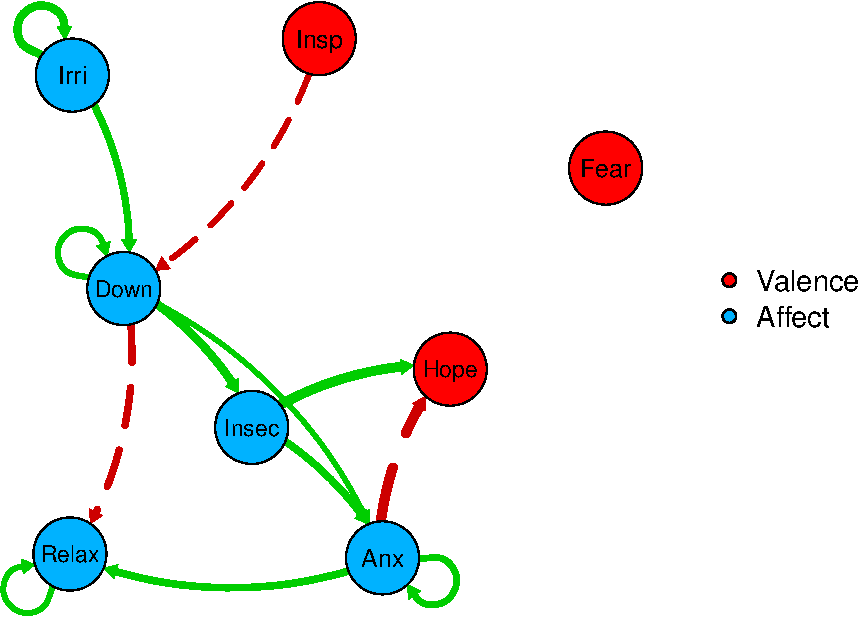
\includegraphics{networkTutorial_files/figure-latex/example1-1.pdf}
\caption{}
\end{figure}

The function `esmNetwork()' is used to run the analyses and build a
network based on these analyses. The function assumes ESM data or a
similar structure. That means that we assume there are persons
(subjects), who have answered a short questionnaires several times a
day, during several days. The intermediate level (days) is not
necessary, and could be absent. The lagged analyses are defined on the
first level, the measurements within days (beeps). The number of lags
can be varied with \enquote{lagn=}, but this will usually be set to 1,
the default value.\\
In the function call \enquote{vars} is a vector with variable names,
which are used to build the netword. The relevant variables can either
be grand-mean centered or centered within groups, which is psecified
with \enquote{centerType}. The centerType option can be a single term
(\enquote{grand-mean} or \enquote{person}) or a vector, which has the
same length as \enquote{vars}, and which specifies for each variable the
type of centering. After \enquote{covs=} the covariates are specified,
which are used in all analyses as covariates, but never as dependent
variables, so they are not plotted in the network. In the multilevel
models all variables can be defined as random effects by setting
\enquote{randomAll=} to true. This means that their slopes are estimated
as random effects. Also, a subset of the variables can be specified as
random effects, using \enquote{randomVars=}. The intercept is usally
estimated as foxed and random effect, but this can be chnaged by the
settin gthe parameters \enquote{fixedIcept} and \enquote{randomIcept} to
FALSE. The layout parameter takes care for the general layout of the
figure. More details can be found in the documentation of the qgraph
function. The \enquote{groups} parameter specifies if different groups
get a different coulour in the figure. The variable labels for the
figure can be specified in the \enquote{labs} parameter. Furthermore,
plmit and solid determine which arrows are drawn in the figure. Finally,
a title can be provided.

With the plot command the plot is drawn in the plots window, as follows.

\begin{Shaded}
\begin{Highlighting}[]
\KeywordTok{plot}\NormalTok{(res}\OperatorTok{$}\NormalTok{output}\OperatorTok{$}\NormalTok{network)}
\end{Highlighting}
\end{Shaded}

\begin{figure}
\centering
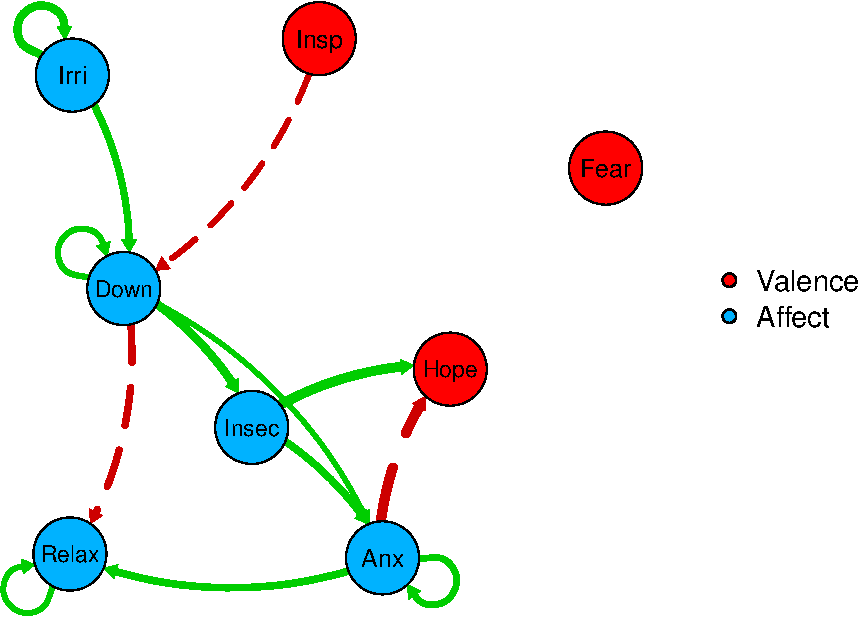
\includegraphics{networkTutorial_files/figure-latex/example1plot-1.pdf}
\caption{}
\end{figure}

\subsection{Indices of centrality}\label{indices-of-centrality}

To better understand the role of the variables in the network several
statistics for a network have been developped, which are called indices
of centrality.

\subsection{Note}\label{note}

We used R (Version 3.5.1; R Core Team, 2018) and the R-packages
\emph{lagnetw} (Version 0.1.4; Verboon, 2019), and \emph{papaja}
(Version 0.1.0.9842; Aust \& Barth, 2018) for all our analyses.

\newpage

\section{References}\label{references}

\begingroup
\setlength{\parindent}{-0.5in} \setlength{\leftskip}{0.5in}

\hypertarget{refs}{}
\hypertarget{ref-R-papaja}{}
Aust, F., \& Barth, M. (2018). \emph{papaja: Create APA manuscripts with
R Markdown}. Retrieved from \url{https://github.com/crsh/papaja}

\hypertarget{ref-Bringmann2018a}{}
Bringmann, L., \& Eronen, M. (2018). Don't blame the model:
Reconsidering the network approach to psychopathology.
\emph{Psychological Review}, \emph{125}(4), 606--615.
doi:\href{https://doi.org/10.1037/rev0000108}{10.1037/rev0000108}

\hypertarget{ref-Costantini2015}{}
Costantini, G., Epskamp, S., Borsboom, D., Perugini, M., Mõttus, R.,
Waldorp, L. J., \& Cramer, A. O. (2015). State of the aRt personality
research: A tutorial on network analysis of personality data in R.
\emph{Journal of Research in Personality}, \emph{54}, 13--29.
doi:\href{https://doi.org/10.1016/j.jrp.2014.07.003}{10.1016/j.jrp.2014.07.003}

\hypertarget{ref-Epskamp2018}{}
Epskamp, S., Borsboom, D., \& Fried, E. I. (2018). Estimating
psychological networks and their accuracy: A tutorial paper.
\emph{Behavior Research Methods}, \emph{50}(1), 195--212.
doi:\href{https://doi.org/10.3758/s13428-017-0862-1}{10.3758/s13428-017-0862-1}

\hypertarget{ref-R-base}{}
R Core Team. (2018). \emph{R: A language and environment for statistical
computing}. Vienna, Austria: R Foundation for Statistical Computing.
Retrieved from \url{https://www.R-project.org/}

\hypertarget{ref-R-lagnetw}{}
Verboon, P. (2019). \emph{Lagnetw: Lagged networks for esm data}.

\endgroup


\end{document}
